\section{Urgensi Kriptografi dalam Teknologi Informasi}
\label{sec:urgensi}

Kriptografi bukan sekadar teori, melainkan inti dari keamanan siber. Pertanyaan yang
wajar diajukan seorang mahasiswa adalah: seberapa nyata akibat kelalaian di bidang
ini? Jawabannya dapat ditemukan pada rentetan peristiwa yang terjadi di Indonesia
sendiri, dan justru karena kedekatan itulah bagian ini disusun agak panjang.

\subsection{Kebocoran Data di Indonesia}

Pada Mei 2021, data BPJS Kesehatan dilaporkan bocor dan diperjualbelikan. Jumlah
data yang ditawarkan mencapai 279 juta, memuat NIK, nama, alamat, nomor telepon,
surel, hingga foto. Data itu dijual di Raid Forums dengan harga 0,15 BTC, yang saat
itu setara Rp70--80 juta. Langkah pemerintah menyusul kemudian: akses unduhan
ditutup, situs Raid Forums diblokir, dan investigasi dijalankan. Yang perlu
dicermati, harga jualnya sangat murah dibandingkan kerugian yang ditimbulkan; bagi
penyerang, biaya memperoleh data semacam itu memang rendah bila sejak awal tidak
dilindungi.

Kebocoran serupa sebenarnya sudah berulang. Pada tahun 2020 tercatat 91 juta data
pengguna dan 7 juta data \textit{merchant} Tokopedia, 2,3 juta data pemilih Pemilu
2014 pada KPU, serta 250 ribu data pasien Covid-19. Daftarnya berlanjut: dugaan
kebocoran data pemilih Pemilu 2014 dan kebocoran sertifikat vaksin; kebocoran
1,64 terabita data Kementerian Pertahanan; serta 1,5 TB data nasabah Bank Syariah
Indonesia yang dibobol kelompok peretas LockBit 3.0 pada Mei 2023. Rentetan kejadian
ini menunjukkan bahwa persoalannya bukan kecelakaan tunggal, melainkan kelemahan
yang sistemik.

Dari rentetan itu muncul kesadaran akan pentingnya regulasi. Masyarakat berhak
mengetahui tujuan penggunaan datanya dan berhak meminta penghapusan data kepada
pengelola; sebaliknya, pengelola wajib melakukan mitigasi terhadap kebocoran dan
dapat dikenai sanksi atau denda bila gagal. Kriptografi adalah salah satu sarana
teknis terpenting untuk memenuhi kewajiban itu, sebab tanpa enkripsi yang memadai,
mitigasi hanya bersifat administratif.

Perlu ditekankan bahwa kasus-kasus di atas pada umumnya bukan kegagalan memecahkan
algoritma kriptografi yang kuat. Yang biasanya terjadi adalah kunci yang tidak
dikelola dengan benar, basis data yang tersimpan tanpa enkripsi (\textit{encryption
at rest} yang diabaikan), maupun kredensial yang bocor. Inilah sebabnya bagian
berikutnya menekankan bahwa keamanan sistem jauh lebih luas daripada sekadar
memilih algoritma.

\subsection{Penyadapan Komunikasi}

Selain kebocoran data, penyadapan komunikasi juga menjadi persoalan nyata. Dua
contoh yang banyak dibicarakan di Indonesia adalah penyadapan kantor Kedutaan Besar
RI di Yangon, Myanmar, yang oleh Menteri Luar Negeri ketika itu dinilai melanggar
Konvensi Wina karena mengganggu fasilitas kedutaan dan menyangkut masalah
kerahasiaan; serta dugaan penyadapan telepon Presiden Susilo Bambang Yudhoyono oleh
pemerintah Australia pada tahun 2013, yang membuat Indonesia memanggil pulang
dubutnya dari Canberra untuk berkonsultasi. Dalam pernyataan resminya, pemerintah
menyebut tindakan itu melanggar privasi individual dan hak asasi manusia.

Kasus-kasus diplomatik semacam ini memperlihatkan bahwa penyadapan tidak terbatas
pada pelaku kejahatan. Negara pun melakukannya, dan sasarannya dapat berupa
saluran komunikasi tingkat tertinggi. Konsekuensinya, perlindungan tidak dapat
diserahkan kepada asumsi bahwa saluran komunikasinya tidak menarik perhatian
siapa pun.

Pada tingkat yang jauh lebih dekat dengan kehidupan sehari-hari, nilai-nilai
seperti WikiLeaks --- pembocoran dokumen Perang Afghanistan pada Juli 2010, 400 ribu
dokumen Perang Irak pada Oktober 2010, dan kawat diplomatik Amerika Serikat pada
November 2010 --- menunjukkan bahwa begitu data rahasia tersimpan dalam bentuk yang
dapat dibaca, kebocorannya hanya menunggu waktu.

\subsection{Keamanan Transaksi Elektronik}

Kriptografi juga menjadi tulang punggung transaksi elektronik. Penggunaan
HTTPS/TLS dalam perbankan daring dan niaga elektronik menjamin privasi dan
otentikasi sekaligus: nasabah yakin berbicara dengan peladen yang benar, dan isi
transaksinya tidak dapat dibaca pihak yang menyadap di tengah jalan. Tanpa
keduanya, sistem pembayaran elektronik tidak akan pernah memperoleh kepercayaan
publik. Pembahasan teknis mengenai bagaimana jaminan itu dibangun disajikan pada
Bab~\ref{chap:tanda-tangan-pki}.

\subsection{Lembaga Terkait Kriptografi di Indonesia}

Di Indonesia, kriptografi tidak hanya menjadi kajian akademis tetapi juga urusan
kenegaraan. Lembaga yang menanganinya antara lain:
\begin{enumerate}
    \item \textbf{Badan Siber dan Sandi Negara (BSSN)}, yang merupakan penggabungan
          Lembaga Sandi Negara (Lemsaneg) dengan Direktorat Jenderal Aplikasi
          Informatika (Aptika) Kementerian Komunikasi dan Informatika.
    \item \textbf{Politeknik Siber dan Sandi Negara (PSSN)}, yang menyelenggarakan
          pendidikan vokasi di bidang persandian.
\end{enumerate}

Selain itu terdapat \textbf{Museum Sandi} di Yogyakarta, yang beralamat di Jalan
Faridan Muridan Noto Nomor 21, Kota Baru, Yogyakarta. Museum ini dikatakan sebagai
satu-satunya museum sandi di Indonesia, bahkan di dunia, dan di dalamnya terdapat
berbagai koleksi alat sandi yang pernah digunakan di Indonesia, termasuk mesin
sandi SN-101. Bagi mahasiswa yang ingin melihat langsung wujud mesin-mesin yang
dibahas dalam buku ini, museum tersebut layak dikunjungi.

\subsection{Tantangan Masa Depan}

Kriptografi sebagai bidang ilmu tidak berhenti berkembang. Sejumlah tantangan yang
kini menonjol antara lain sebagai berikut.

\begin{itemize}
    \item \textbf{Kriptografi ringan} (\textit{lightweight cryptography}), yaitu
          primitif kriptografi yang dirancang agar hemat daya, memori, dan siklus
          komputasi sehingga layak dipasang pada perangkat Internet of Things.
          Gambar~\ref{fig:lightweight-cryptography-iot} memperlihatkan cabang-cabang
          primitifnya: block cipher ringan, stream cipher ringan, fungsi hash
          ringan, dan ECC.
    \item \textbf{Kriptografi pasca-kuantum} (\textit{post-quantum cryptography}),
          yaitu algoritma yang diharapkan tetap aman terhadap komputer kuantum.
          Algoritma Shor mengancam RSA dan ECC, sehingga dikembangkan keluarga baru
          berbasis \textit{hash}, kode, multivariat, dan kisi (\textit{lattice}).
    \item \textbf{Kriptografi berbasis kecerdasan buatan dan serangan berbantuan
          AI}. Pembelajaran mesin dapat dipakai untuk mempercepat kriptanalisis
          maupun untuk merancang primitif baru.
    \item \textbf{\textit{Selective encryption} untuk data multimedia}, yaitu
          enkripsi yang hanya menyandikan bagian terpenting dari aliran video
          sehingga hemat sumber daya namun tetap melindungi isinya.
\end{itemize}

\begin{figure}[htbp]
    \centering
    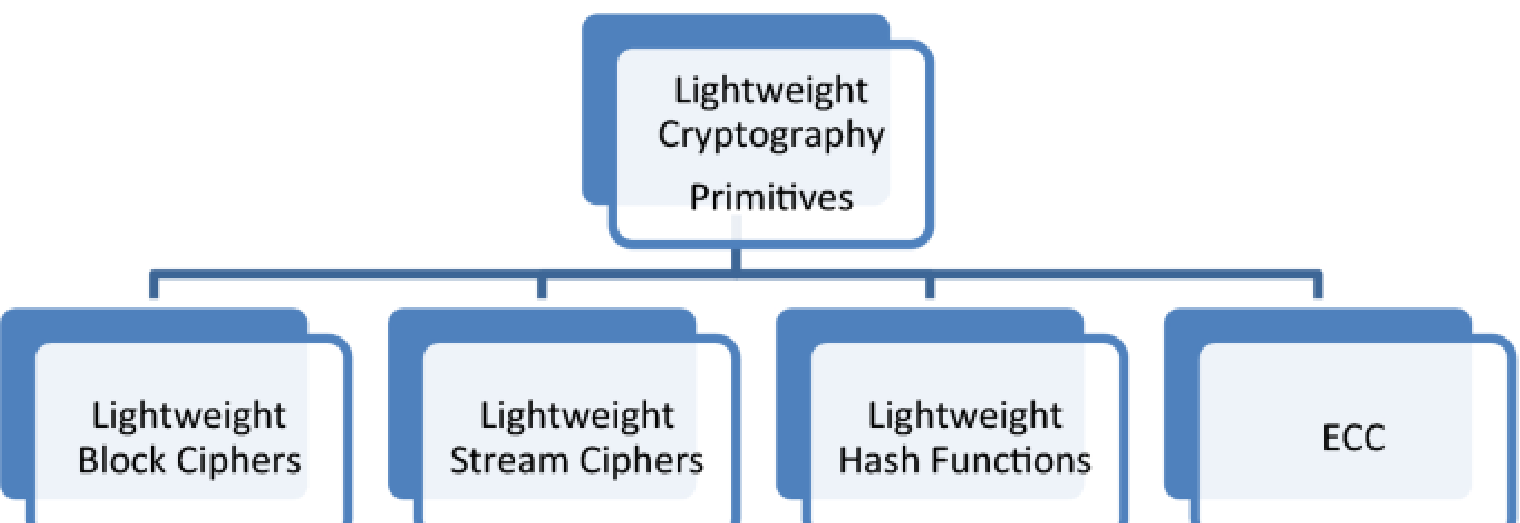
\includegraphics[width=0.88\linewidth, height=0.5\textheight, keepaspectratio]{figures/lightweight-cryptography-iot.png}
    \caption{Cabang primitif pada kriptografi ringan untuk perangkat Internet of Things: \textit{block cipher}, \textit{stream cipher}, fungsi hash, dan ECC}
    \label{fig:lightweight-cryptography-iot}
    \sumber{Munir, \textit{IF4020 Kriptografi}, ITB.}
\end{figure}

\begin{figure}[htbp]
    \centering
    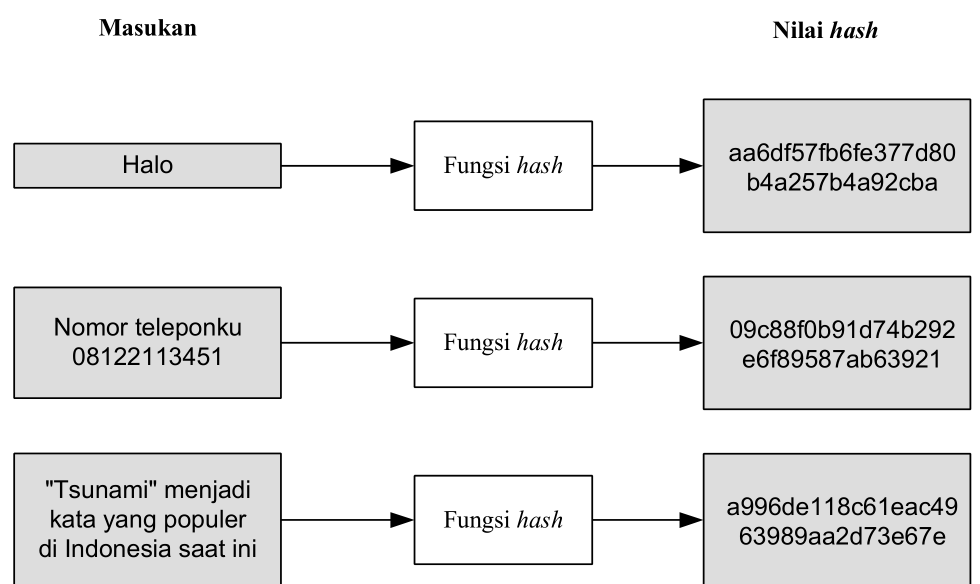
\includegraphics[width=0.8\linewidth, height=0.55\textheight, keepaspectratio]{figures/fungsi-hash-integritas.png}
    \caption{Fungsi hash memetakan masukan berukuran bebas menjadi nilai hash berpanjang tetap; masukan yang berbeda menghasilkan nilai hash yang berbeda}
    \label{fig:fungsi-hash-integritas}
    \sumber{Munir, \textit{IF4020 Kriptografi}, ITB.}
\end{figure}
